\documentclass[12pt]{article}

% Load necessary packages
\usepackage{geometry}
\usepackage{setspace}
\usepackage{natbib}
\usepackage{graphicx}
\usepackage{amsmath}
\usepackage{amssymb}
\usepackage{caption}
\usepackage{subcaption}
\usepackage{hyperref}
\usepackage{graphicx}
\usepackage{float}

% Set page margins
\geometry{margin=1.1in}

% Set line spacing
\doublespacing

% Title and author information
\title{Exploring the relationship between mother household headship and child vaccination rate in Nepal
}
\author{Prabidhik KC\thanks{Harvard University, Cambridge, USA. Email: \href{mailto:prabidhik_kc@college.harvard.edu}{prabidhik_kc@college.harvard.edu}}}

% Date
\date{May 7, 2023}

\begin{document}

% Title page
\maketitle

% Abstract
\begin{abstract}
I exploit the differences in family member absentees caused by the foreign employement to estimate the effect of mother household headship on child vaccination rate. Using instrumental variable method and data from Nepal Social Inclusion Survey (NSIS) 2018, I find that there is no statistically significant affect on child vaccination rate if the household head is mother instead of father. Even after controlling for education, log wage, ethnicity, I do not find any significant effect in bacterial vaccination and viral vaccination.
\end{abstract}

% Introduction
\section{Introduction}
In low income countries, communicable disease is far more likely to be a cause of death than a noncommunicable disease. 6 of the top 10 causes of death remain such communicable diseases in low income countries, with Tuberculosis, HIV/AIDS and malaria all remaining in the top 10 (WHO, 2019). Thus, childhood vaccination is a crucial component of public health programs especially as a profound measure to reduce deaths from such diseases, notably in the developing countries like Nepal. According to Ministry of Health and Population, Nepal started providing BCG vaccine to all infants in free of cost (National Immunization Program) since 2005, pneumococcal vaccine since  2019, Oral Polio and DPT since 1979, Rubella in 2018. Despite this availability of free vaccines, the vaccinations coverage in Nepal is not yet full capacity, shown in the map of Nepal below in two categories: viral vaccination which includes Oral Polio, DPT, and Rubella and bacterial vaccine which includes BCG and Pneumococcal vaccine, with each 14 zones: the zone Karnali is not included because of lack of data, which puts children at a risk of preventable diseases. Previous researches have identified various factors that affects vaccination rates including socioeconomic conditions, maternal education, access to health care to mention few. However, the impact of maternal headship on vaccination rate has received less attention in the literature. This research aims to fill this gap by examining whether mother as a household head affects child vaccination rate in Nepal, using Nepal Inclusion Social Survey (NSIS) 2018. The findings of this study will provide insights into the role of household headship improving vaccination coverage and inform policies to promote child health care in Nepal.


\begin{figure}[h]
    \centering
    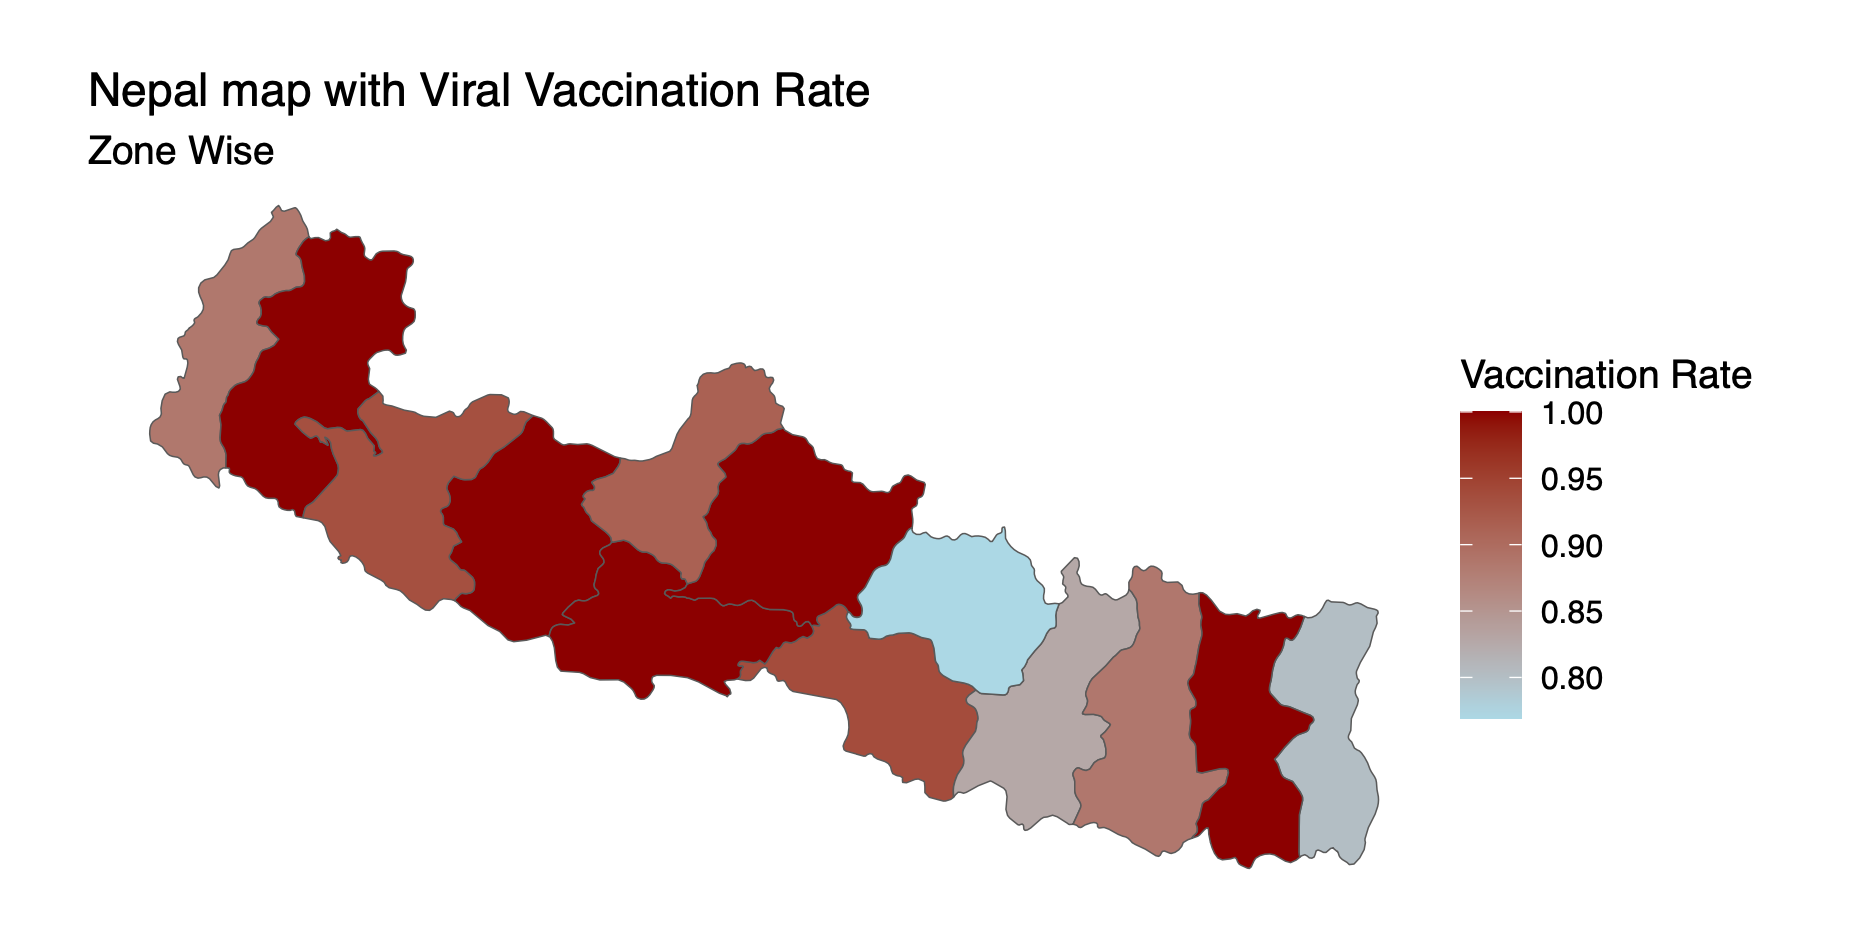
\includegraphics[width=1\textwidth]{viral.png}
    \caption{Viral Vaccination rate in different zones of Nepal}
    \label{Viral Vaccination rate in different zones of Nepal}
\end{figure}

\begin{figure}[h]
    \centering
    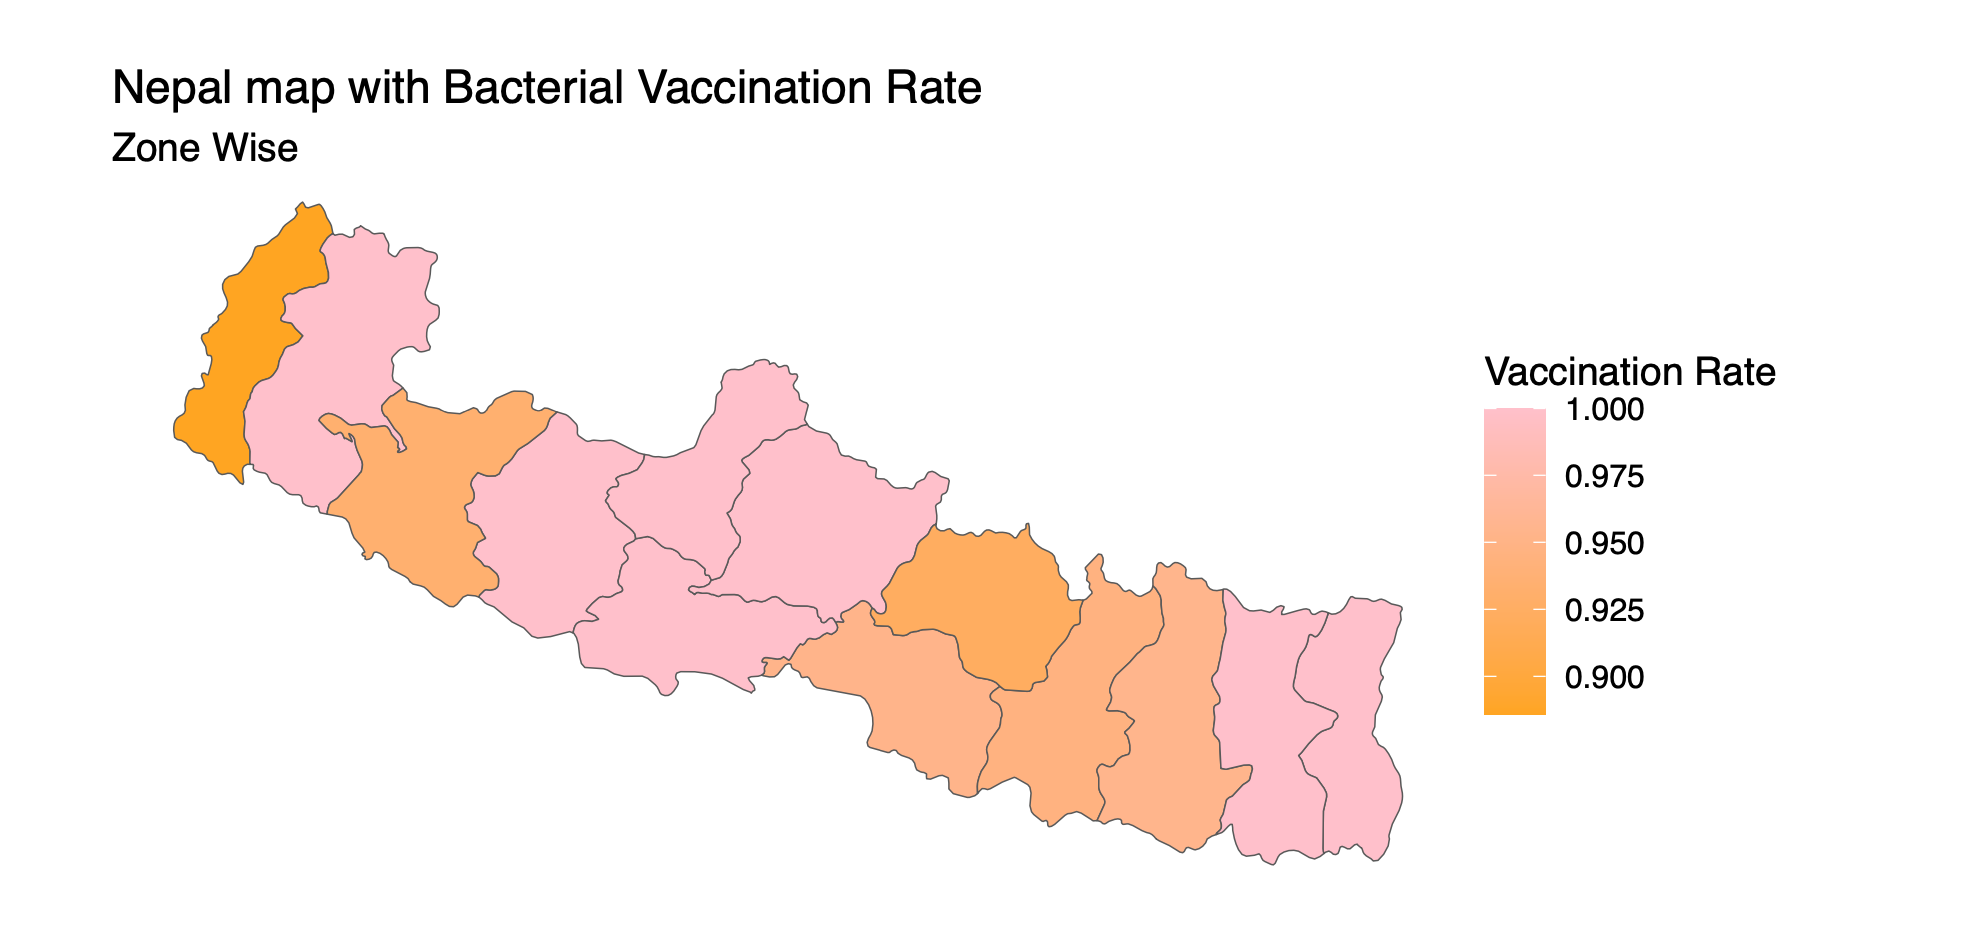
\includegraphics[width=1\textwidth]{bacterial.png}
    \caption{Bacterial Vaccination rate in different zones of Nepal}
    \label{Bacterial Vaccination rate in different zones of Nepal}
\end{figure}

% Literature Review
\section{Literature Review}
Vaccination is a pivotal preventive measure, particularly for the children, as it helps them protect them against several diseases. The World Health Organization estimates that the vaccination prevents approximately 2-3 million deaths per year. However, despite these proven efficacy of vaccines, there are still gaps in vaccination coverages in many parts of the world, specifically in low and middle income countries (Yousufzhai et. al, 2018). Nepal is one such country where vaccination rates are still low with only 77\% of children, as shown in the map above, aged 12-23 months having received all the vaccinations (Ministry of Health and Population, 2019).

The literature on the relationship between household headship and child health outcomes is mixed. Some studies suggest that having a female household headship is associated with a lower child vaccination rate due to socioeconomic status and limited access to health care services (Burgard \& reiman, 2006; Fulu et al., 2017, Sharma \& Reichenbach, 2018). 

In the context of Nepal, few studies have examined the relationship between the household headship and child vaccination rates. One study found that household with female headship were less likely to vaccinate their children due to lower education level and socioeconomic status (Kamiya et. al, 2017). However, this study did not control for other important factors that may have influenced vaccination rate such as access to health care and maternal-decision making power. Therefore, further research is necessary to understand the household headship and children vaccination rate in Nepal.

The NSIS data from 2018 provides us a unique opportunity to examine this relationship. The dataset includes detail information on household composition, socioeconomic status, and child health outcomes, absentee population allowing for the comprehensive analysis of the factors related with the child vaccination rate. By exploring the relationship between household headship and child vaccinations rate in Nepal, this research aims to provide valuable insights into the factors that affect child vaccination rate.


% Data 
\section{Data}
In my study, I use data from Nepal Social Inclusion Survey (NSIS) 2018. NSIS is a survey dataset which is conducted as a Study On Social Inclusion In Nepal (SOSIN) by Central Department of Anthropology, Tribhuwan University.  The dataset reports information on various socio-economc indicators of household and individuals in Nepal. It includes information on different characteristics within household information, health and social security, work and livelihood, language and education, social, cultural and gender relations, inclusive governance, women's empowerment and reproductive health.
The summary statistics of the final data that I used is given below:

\begin{figure}[H]
    \centering
    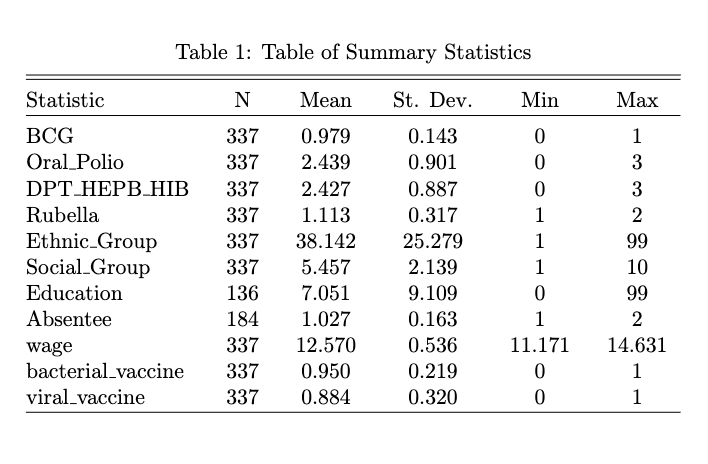
\includegraphics[width=0.65\textwidth]{summary_statistcs.png}
    \caption{Table 1}
    \label{Table of Summary Statistics}
\end{figure}

I pooled the dataset from parent NSIS 2018 datasets which was further divided into sub datasets based on different demographic and economics sections. I merged the datasets which included the information that I required for this questions such as data on vaccinations, family income, education, ethnic groups and absentee population.
I then assigned 1 to each of BCG, Pneumococcal, Oral Polio, DPT/HEPB/HIB, Rubella if they had been given to their child else they else 0 was assigned. These vaccinations were further divided into bacterial vaccine and viral vaccine based on the characteristics of the cause of the disease that we are interested. They are further assigned 1 if each of bacterial or viral vaccines were administered else 0 was assigned. I also restrict the data to those families that had at least one absentee population. The absentee population is defined as anyone who is not present in the family because of foreign employment (within country or outside country) so that it can be used as an instrument. Families with missing information for any of the variables of our question were omitted. The final dataset has 337 observations out of which approximately 84\% were households with female head. \footnote{We have selected the families with at least one absentee population}. Table 1 summarizes the above dataset. We see that on average 95\% of the family had given the child full vaccinations for a bacterial disease and 88\% had given full vaccinations for viral disease.
% Methods
\section{Methods}
I use instrumental variable method to study the causal relationship between female household headship and child vaccination rate. The absentee population is defined as the instrument. In this paper, absentee population is defined as the member of the family who is away from home for the employment. I wish to estimate the following regression model:
\begin{align}
    y_i = \beta_0 + \beta_1 x_i + \eta_i
\end{align}
In this regression, we are interested in $\beta_1$ as our coefficient of interest. But the problem is that there can be a problem of edogeneity as the error term is possibly correlated with our variable of independent variable. So, I come up with the first stage regression model:
\begin{align}
    x_i = \pi_0 + \pi z_i + \nu_i
\end{align}
where $\pi_0 + \pi z_i$ is the component of $x_i$ that is explained by $z_i$ while $\nu_i$ is the component that cannot be explained by $z_i$ and exhibits correlation with $\nu_i$.
where I have assumed that the following assumptions holds:\\
(i) Exogeneity: the absentee population is not related with the error term in equation (1).\\
(ii) Relevance: The household head being a female is correlated with the absentee population.
(iii) Exclusion restriction: the absentee population is not correlated with vaccination rate of the child. absentee population is correlated with child vaccination rate except through their effect on the endogenous variable of interest.\\
(iv) Monotonicity: The absentee does not have effect on the outcome variable other than through their effect on the endogenous variable of interest.\\
(v) Validity: The absentee population is not a subject to measurement error or other forms of bias.

Given that there is an absentee in the family (the dataset that we are interested in), male absentee consists massive 90.24 \% while female absentee consists only 9.76\%. So, in an overall data, male consists 83.2\% and female consists 16.8\% as head of the household. In our dataset female as a household consists 68.4\%. So it becomes obvious that when there is a absentee in a family, mother is most likely to be the head of the household. {this much percentage vaccination rate overall and when there is an absentee in the family, this much}. So, we can conclude that there is not much a correlation of being absentee to the child vaccination rate. We will be testing the limitations of these assumptions later, but we can argue that our instrument for the analysis is a valid instrument. The procedure of our instrumental variable method can be summarized in the figure below:

\begin{figure}[H]
    \centering
    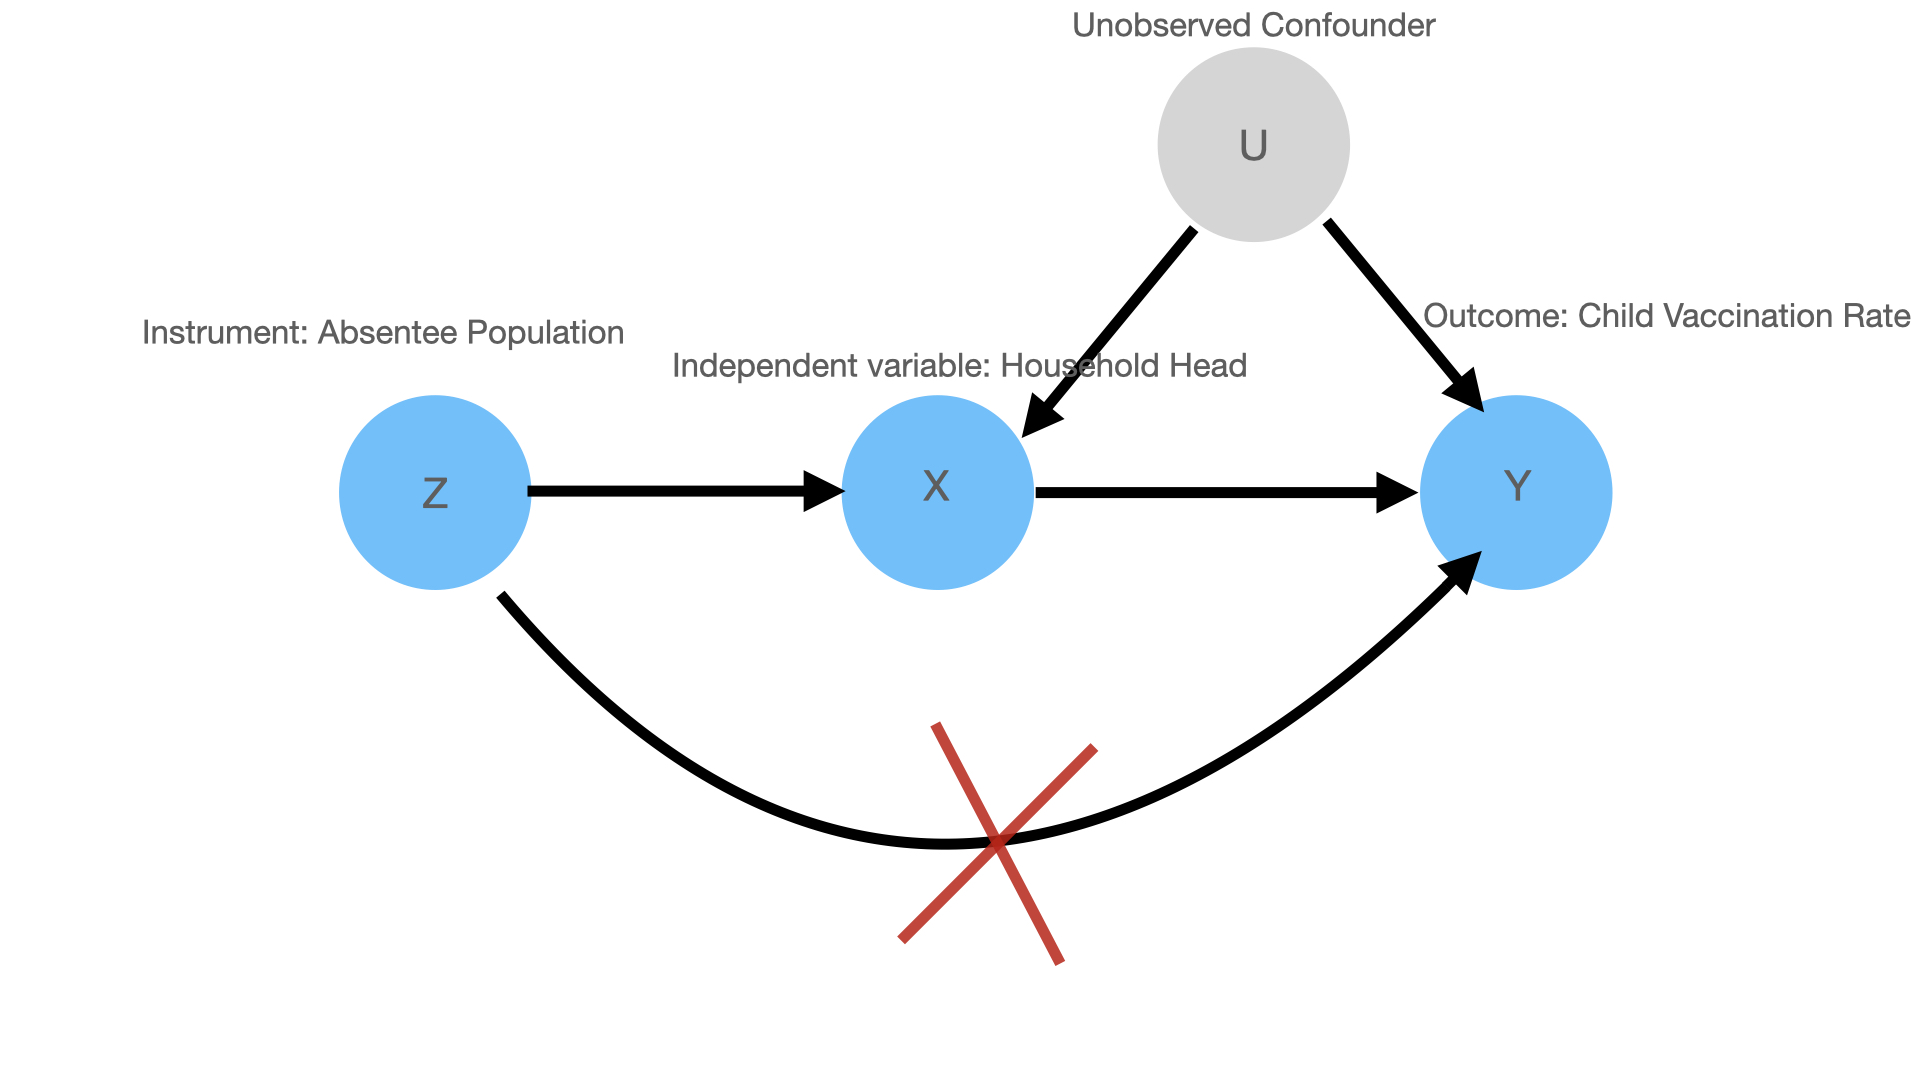
\includegraphics[width=1.0\textwidth]{iv_model.001.jpeg}
    \caption{Use of instrumental variable}
    \label{Table of Summary Statistics}
\end{figure}

As our vaccination rate is further divided into viral vaccination rate and bacterial vaccination rate, I apply the same method and instrument in both the cases with outcome being either bacterial vaccination rate or viral vaccination rate.

The reduced form regression that I use is:

\begin{align}
    y_i = \mu_0 + \mu z_i + \theta_i
\end{align}


We then divide the beta coefficient obtained from the reduced form regression by the beta coefficient obtained from first stage regression to find the beta coefficient of interest. I controlled for potential confounding variables by including them as covariates in our regression model. Specifically, I included variables: log wage, education, social group, ethnic group to account for their potential effects on the outcome variable.

% Results
\section{Results}
Table 2 summarizes the results of my regression which includes characteristics like education, log wage, social group belonging as controls in addition to the instrument. The instrumental variable regression suggests that an increase in female household head by one unit has a causal effect of increment in 0.61 child bacterial vaccination rate when education, log wage, and social group are not controlled, and increment of 0.41 child bacterial vaccination rate when these characteristics are controlled. However as the standard errors of these beta coefficients are extremely high, the results are statistically insignificant, meaning that we cannot make any certain conclusions that if there is any significant effect of mother being a household head is likely to cause higher child bacterial vaccination rate.
Another variable of interest is log wage. One percent increase in wage hazs an effect of increase of bacterial vaccination rate (0.04*100) = 4\% increase in bacterial vaccination rate. However, this coefficient is also statistically insignificant.

Similarly, table 3 summarizes the results of my regression on viral vaccination rate, which also includes characteristics like education, log wage, social group as well as ethnic group belonging controls in addition to the instrument. The instrumental variable regression suggests that an increase in female household head by one unit has a causal effect of increment in 0.61 child viral vaccination rate when education, log wage, ethnic and social group are not controlled, and increment of 3.89 child viral vaccination rate when these characteristics are controlled. However as the standard errors of these beta coefficients are extremely high, the results are statistically insignificant, meaning that we cannot make any certain conclusions that if there is any significant effect of mother being a household head is likely to cause higher child viral vaccination rate. Some other variable of interests are education and social group. It seems that education is directly causing higher and social group is lower viral vaccination rate. However, just as earlier, these coefficients are statistically insignificant.

\begin{figure}[H]
    \centering
    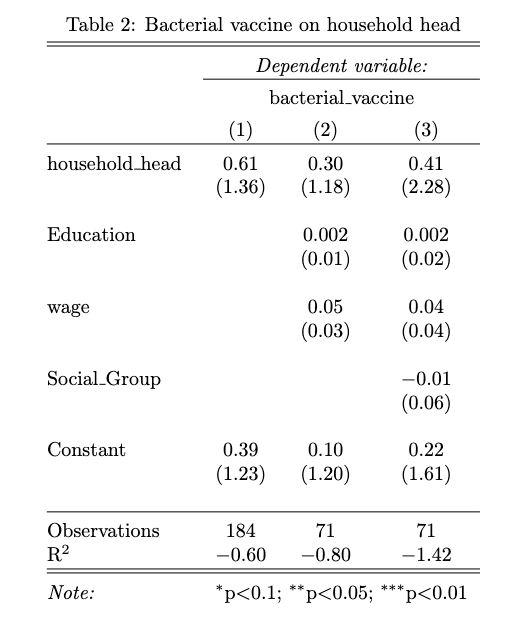
\includegraphics[width=0.9\textwidth]{bacterial_vaccine_reg.png}
    \caption{Use of instrumental variable}
    \label{Table of Summary Statistics}
\end{figure}

\begin{figure}[H]
    \centering
    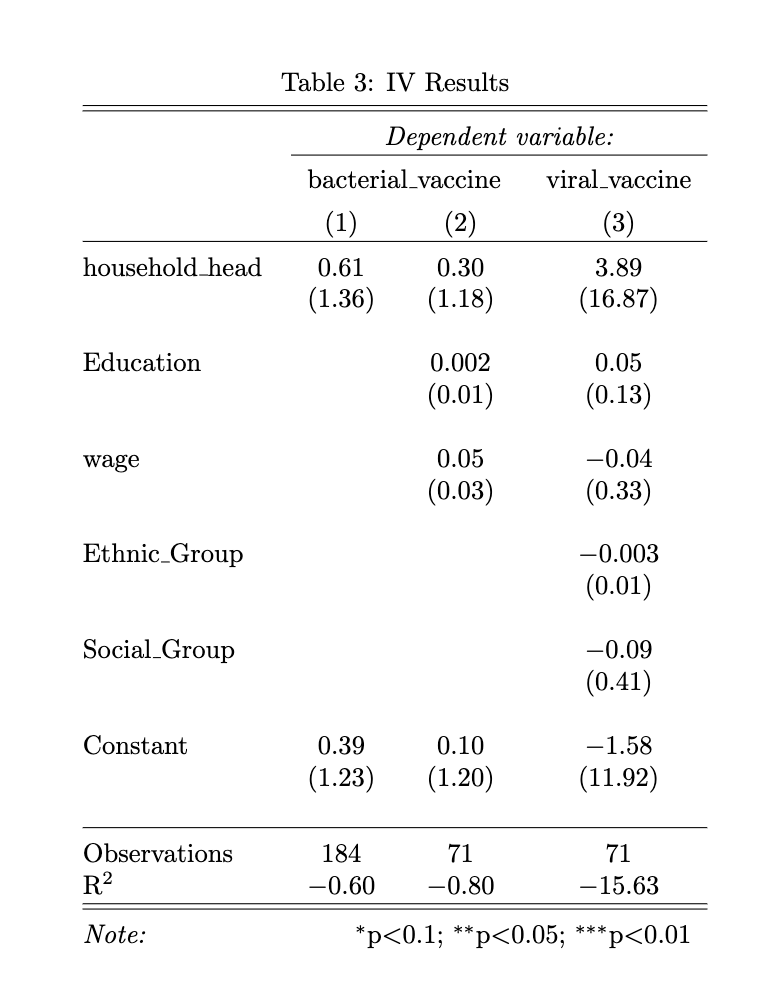
\includegraphics[width=0.9\textwidth]{viral_vaccination.png}
    \caption{Use of instrumental variable}
    \label{Table of Summary Statistics}
\end{figure}
% Discussion
\section{Discussion}
This study aimed to investigate the relationship between mother household headship and child vaccination rates in Nepal. Using data from the Nepal Social Inclusion Survey 2018 and instrumental variable method, I found that there was no statistically significant difference between the effectiveness of mother household headship and father household headship in ensuring higher child vaccination rate.\\
These findings are consistent with few previous studies that have examined the impact of female decision-making power on health outcomes . For instance, a study by Ahmed \& Hasan (2008), Schuler \& Hashemi (1994), Bloom, Wypij \& Das Gupta (2001) provide evidence that household headship by either parent has similar effects on health outcomes. Similarly, our results suggest that in the context of Nepal, the gender of the household may not be as important as other factors such as access to health care in determining child vaccination rate. However, Nisar et al., (2018), (Kanmiki et al. (2019), (Akmatov et al. (2015) suggest that female household headhsip is likely to have higher vaccination rate of children. These inconsistencies show the need for further research and also the importance of other important factors such as education, income, cultural, geographical characteristics while trying to understand these questions.

% Limitations
\section{Limitations}
While the study suggests that there is no significant effect on mother household headship in child vaccination outcome, this study has several limitations that should be considered while interpreting the results. The study sample was limited to 337 observations, which may limit the statistical power of the analysis and lead to imprecise estimates. Further studies with larger sample size may be able to provide more robust and accurate results. Secondly, the study focused on the relationship between household headship and child vaccination rates and although important characteristics like education, income, and ethnicity were accounted for, other potential determinants such as healthcare access and health awareness were not accounted for. Finally, the study was conducted in the specific context of Nepal, where cultural and social norms differ from other countries. Therefore, the results may not be directly applicable to other settings.

% conclusion

\section{Conclusion}
In conclusion, this study used an instrumental variable method to examine the relationship between mother household headship and child vaccination rate in Nepal. The findings did not show any statistically significant difference between mother and father household headship in terms of their effectiveness in improving child vaccination rates. This suggests that both parents can play an equally important role in promoting child health through vaccination.\\

Although this study provides insights into the potential role of the household headship in improving child vaccination rates, it has several limitations as discussed in earlier section. Future research could use larger sample sizes and longitudinal data to explore the relationship between household headship and child health outcomes further. Additionally, a wider range of variables in the analysis could provide more insight into the complex factors that affect child vaccination rates in Nepal.\\

Overall our study adds to the growing body of literature on the role of female decision-making power on child health outcomes.  It highlights the importance of considering household dynamics in the context of child health outcomes. Policymakers and public health practitioners should continue to focus on interventions that promote vaccination uptake among both mothers and fathers to improve child health outcomes in Nepal.\\

% References

\begin{center}
\textbf{\fontsize{25pt}{1.5em}\selectfont
Work Cited}
\end{center}
\begin{itemize}
    \item Center Department of Anthropology, Tribhuwan University, National Social Inclusion Survey (2018)
    \item WHO. (2019). World health statistics 2019: Monitoring health for the SDGs, sustainable development goals. World Health Organization.
    \item National Immunization Program Nepal. (n.d.). Retrieved May 7, 2023, from https://nip.org.np/
    \item Ministry of Health and Population (2019). National Immunization Program. Retrieved from https://nepal.un.org/en/37286-national-immunization-programme-nip
    \item Burgard, S. A., \& Reimann, J. O. (2006). Widowhood, Divorce, and Loss of Long-Term Care Insurance: A Panel Study of Older Women. Journals of Gerontology Series B: Psychological Sciences and Social Sciences, 61(4), S223-S232.
    \item Fulu, E., Miedema, S., Roselli, T., McCleary-Sills, J., \& Xianhong, L. (2017). Women's and men's reports of past-year prevalence of intimate partner violence and rape and women's risk factors for intimate partner violence: a multicountry cross-sectional study in Asia and the Pacific. PLoS medicine, 14(9), e1002381.
    \item Sharma, N., \& Reichenbach, L. (2018). Gender inequality in immunisation status among children under five years of age living in Nepal. Sage Open Medicine, 6, 1-8.
    \item Kamiya, Y., Yoshimura, Y., Islam, M. A., Matsuura, A., Kuroiwa, C., Shimizu, K., \& Wakai, S. (2017). Factors affecting immunization status among children under five years of age in Nepal: a multilevel analysis. BMC public health, 17(1), 1-10.
    \item Ahmed, S. M., \& Hasan, M. M. (2008). Do mothers or fathers have greater influence on preventing malnutrition among children under the age of 5 in slum areas of Bangladesh?. Food and Nutrition Bulletin, 29(3), 221-231.
    \item Schuler, S. R.,\& Hashemi, S. M. (1994). Credit programs, women's empowerment, and contraceptive use in rural Bangladesh. Studies in Family Planning, 25(2), 65-76.
    \item Bloom, S. S., Wypij, D., \& Das Gupta, M. (2001). Dimensions of women's autonomy and the influence on maternal health care utilization in a north Indian city. Demography, 38(1), 67-78.
    \item Nisar, N., Mirza, M., Nazir, S., \& Khan, A. (2018). Household decision-making regarding child vaccination and its impact on coverage: findings from low- and lower-middle-income countries. Human Vaccines \& Immunotherapeutics, 14(12), 2939-2945. https://doi.org/10.1080/21645515.2018.1495458
    \item Kanmiki, E. W., Bawah, A. A., Akazili, J., Agorinyah, I. N., Achana, F. S., \& Awoonor-Williams, J. K. (2019). Factors associated with incomplete childhood immunization among residents of the Kassena-Nankana districts of northern Ghana: A case–control study. PloS one, 14(8), e0221383. https://doi.org/10.1371/journal.pone.0221383
    \item Akmatov, M. K., Rizlaine, R., Ellerbroek, L., \& May, J. (2015). Validity of vaccination coverage estimates from health surveys in rural Senegal: A comparison of estimates from household-based versus health facility-based surveys. The American Journal of Tropical Medicine and Hygiene, 92(1), 158-163. https://doi.org/10.4269/ajtmh.14-0479

\end{itemize}



\end{document}
